%\documentclass[conference]{IEEEtran}
\documentclass[12pt]{article}
\usepackage{graphicx,cite,bm,psfrag,amsmath}
\def\mmax{\mathop{\mbox{\scriptsize max}}}
\def\argmin{\mathop{\mbox{arg\,min}}}
\def\argmax{\mathop{\mbox{arg\,max}}}
\newcommand{\defequal}{\stackrel{\mathrm{def}}{=}}
\renewcommand{\vec}[1]{{\ensuremath{\boldsymbol{#1}}}}
\newcommand{\popt}{\ensuremath{P^{(K)}_{opt}}}

\pagestyle{plain}
\usepackage{amsfonts}
\usepackage{algorithm, algorithmic}
\renewcommand{\algorithmicrequire}{ \textbf{Input:}} %Use Input in the format of Algorithm
\renewcommand{\algorithmicensure}{ \textbf{Procedures:}} %UseOutput in the format of Algorithm
% correct bad hyphenation here
%\hyphenation{op-tical net-works semi-conduc-tor}
\usepackage{CJK}
\usepackage{color}
\usepackage{url}
\usepackage{geometry}
\geometry{left=0.55in, right=0.7in, top=0.75in, bottom=0.75in}

\begin{document}
\title{Appendix for SIR-Based Power Control Used in CDMA Systems}
%\author{\IEEEauthorblockN{Wentao Liu, Guanchong Niu and Man-On Pun\IEEEauthorrefmark{3}
%%\IEEEauthorrefmark{3},
%\IEEEauthorblockA{
%School of Science and Engineering\\
%The Chinese University of Hong Kong, Shenzhen\\
%Shenzhen, Guangdong, China, 518172}}}


%\maketitle \thispagestyle{plain}
\pagenumbering{gobble}


% make the title area
\maketitle

\section{Derivation for Eigenvalue problem}
In this system, the $N$ users are distributed in $K$ cells randomly as shown in Fig.\ref{fig:t}.
The users are grouped by calculating the minimal distance on the center of each cell.
\begin{figure}[th]
	\centering
	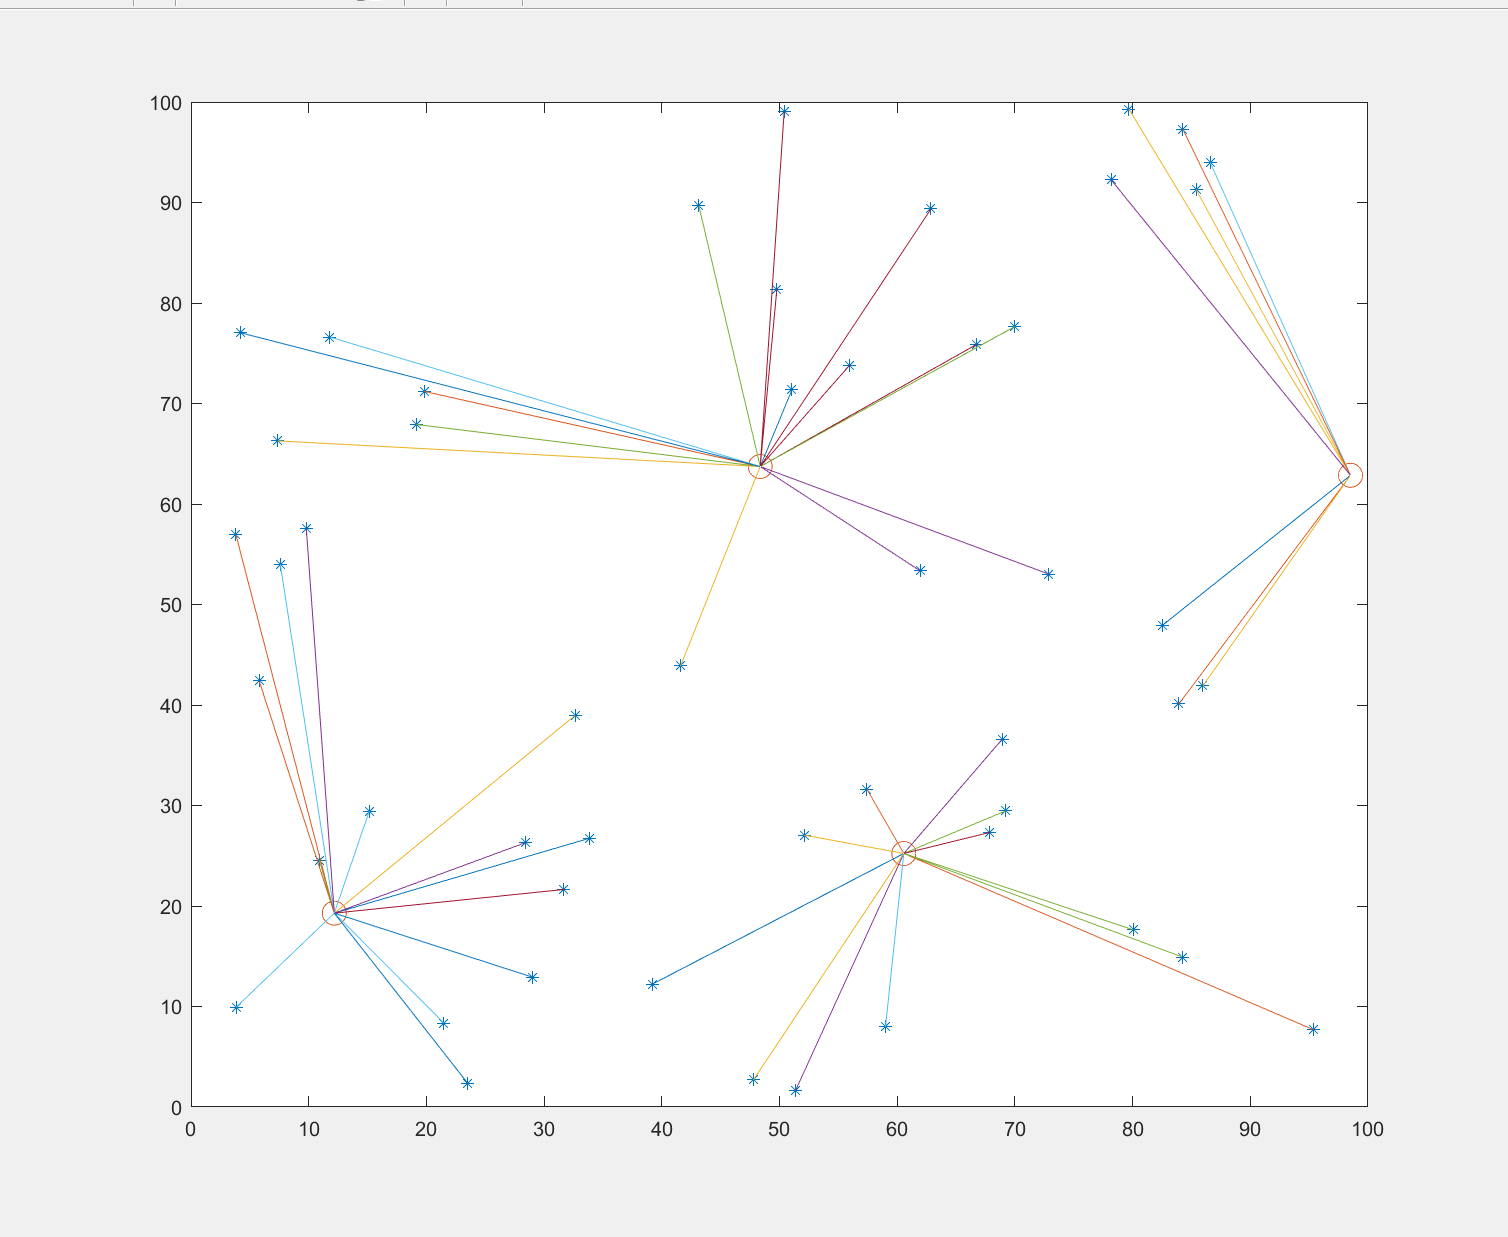
\includegraphics[scale=0.4]{distribution}
	\caption{An example with 50 users and 4 cells.}
	\label{fig:t}
\end{figure}

The pathloss of each user is given by
\begin{equation}
L_{uk} = d_{uk}^3
\end{equation}
where $d_{uk}$ is the distance from $u$-th user to $k$-th center.

The SIR $\gamma_1$ of 1st user in 1st cell, \textit{i.e.} $k_1=1$ can be represented as
\begin{align}\label{gamma}
	\gamma_1 &= \frac{P_1/L_{11}}{\sum_{u\neq 1}^{N}P_{u}/L_{u1}} \nonumber\\
	&= \frac{P_1/L_{11}}{\sum_{u=1}^{N}P_{u}/L_{u1} - P_1/L_{11}} \nonumber\\
	&= \frac{P_1}{L_{11}\sum_{u=1}^{N}P_{u}/L_{u1} - P_1} 
\end{align}

From Eq. \eqref{gamma}, we have
\begin{align}
\frac{\gamma+1}{\gamma}P_1 &= L_{11}\sum_{u=1}^{N}P_{u}/L_{u1} \\
& = L_{11} 
[1/L_{11}, 1/L_{21},\cdots, 1/L_{N1}]
\begin{bmatrix}
P_{1}\\
\cdots \\
P_{N}
\end{bmatrix}\\
&=[1, L_{11}/L_{21},\cdots, L_{11}/L_{N1}]
\begin{bmatrix}
P_{1}\\
\cdots \\
P_{N}
\end{bmatrix}
\end{align}

By applying the balanced SIR algorithm on all users, the problem is formulated as
\begin{align}
\frac{\gamma+1}{\gamma}\bm{p} &= \bm{G}\bm{p}\\
\frac{1}{\gamma}\bm{p} &= (\bm{G}-\bm{I})\bm{p}
\end{align}
where 
\begin{align}
\bm{G} = 
\begin{bmatrix}
1& L_{1k_1}/L_{2k_1}&\cdots& L_{1k_1}/L_{Nk_1}\\
L_{2k_2}/L_{1k_2}& 1&\cdots& L_{2k_2}/L_{Nk_2}\\
\vdots&\vdots&\vdots&\vdots\\
L_{Nk_N}/L_{1k_N}& L_{Nk_N}/L_{2k_N}&\cdots& 1
\end{bmatrix}
\quad
\bm{p} =
\begin{bmatrix}
P_{1}\\
P_{2}\\
\vdots\\
P_N
\end{bmatrix}
\end{align}
where the $k_u,u\in (1, N)$ means that the $u$-th user is distributed to $k$-th cell.

\textbf{Based on the \textit{Perron–Frobenius theorem}, there exists an eigenvector that all the elements are positive. Since $trace(G-I)=0$, there must exist an eigenvalue lager than 0.}

\section{Proof for $\bm{G}^U = (\bm{G}^D)^T$}
 For 1st user in 1st cell, \textit{i.e.} $k_1=1$
\begin{align}\label{gammaD}
\gamma_1 &= \frac{P_1/L_{11}}{\sum_{u\neq 1}^{N}P_{u}/L_{1k_u}} \nonumber\\
&=\frac{P_1/L_{11}}{\sum_{u=1}^{N}P_{u}/L_{1k_u} - P_1/L_{11}} \nonumber\\
&= \frac{P_1}{L_{11}\sum_{u=1}^{N}P_{u}/L_{1k_u} - P_1} 
\end{align}
The SIR for downlink is represented as
\begin{align}
\frac{\gamma+1}{\gamma}\bm{p}^D &= \bm{G}^D\bm{p}^D\\
\frac{1}{\gamma}\bm{p}^D &= (\bm{G}^D-\bm{I})\bm{p}^D
\end{align}
where 
\begin{align}
\bm{G}^D = 
\begin{bmatrix}
1& L_{1k_1}/L_{1k_2}&\cdots& L_{1k_1}/L_{1k_N}\\
L_{2k_2}/L_{2k_1}& 1&\cdots& L_{2k_2}/L_{2k_N}\\
\vdots&\vdots&\vdots&\vdots\\
L_{Nk_N}/L_{Nk_1}& L_{Nk_N}/L_{Nk_2}&\cdots& 1
\end{bmatrix}
\quad
\bm{p}^D =
\begin{bmatrix}
P_{1}\\
P_{2}\\
\vdots\\
P_N
\end{bmatrix}
\end{align}
%\bibliography{PCAref}
%\bibliographystyle{IEEEtran}
\end{document}


